\documentclass[a4paper,12pt]{article}
\usepackage[utf8]{inputenc}
\usepackage{amsmath}
\usepackage{amsfonts}
\usepackage{amssymb}
\usepackage{graphicx}
\usepackage{caption}
\usepackage{subcaption}
\usepackage{float}
\usepackage{siunitx}
\usepackage{booktabs}
\usepackage{hyperref}

\title{Reticolo}
\author{Francesco Giuseppe Minisini, Mattia Monzani, Gabriele Turi}
\date{January 13, 2025}

\begin{document}

\maketitle
\hrule
\vspace{9pt}
\begin{abstract}
    \noindent
    Utilizzando lo spettrometro a reticolo sono state misurate le lunghezze d’onda dello spettro di emissione del mercurio, ottenendo i seguenti risultati: \( \lambda_{\text{rosso}} = (6240 \pm 3) \, \text{\AA} \), \( \lambda_{\text{giallo1}} = (5791.5 \pm 1.6) \, \text{\AA} \), \( \lambda_{\text{giallo2}} = (5770.8 \pm 1.7) \, \text{\AA} \), \( \lambda_{\text{verde}} = (5461.1 \pm 2.0) \, \text{\AA} \), \( \lambda_{\text{azzurro}} = (4963.5 \pm 2.7) \, \text{\AA} \), \( \lambda_{\text{indaco}} = (4359.6 \pm 1.8) \, \text{\AA} \), \( \lambda_{\text{violetto1}} = (4079.9 \pm 2.8) \, \text{\AA} \), \( \lambda_{\text{violetto2}} = (4046.3 \pm 2.2) \, \text{\AA} \). 
    In seguito è stato misurato il potere dispersivo \( D \) e risolutivo \( R \) dell’apparato, ottenendo \( D = (1.0343 \pm 0.0003) \times 10^6 \, \text{rad/m} \) per alcune coppie di lunghezze d'onda e \( R = 7318 \pm 6 \) per il doppietto del sodio. L'ortogonalizzazione del reticolo e il calcolo del passo \( d \) \((3.3790 \pm 0.0007) \, \mu\text{m}\) hanno confermato la precisione del sistema sperimentale. I risultati mostrano una compatibilità superiore al \(19\%\) con i valori noti, evidenziando l'efficacia del metodo utilizzato.
\vspace{20pt}
\hrule
\end{abstract}
\vspace{2 pt}


\section{Messa a punto dell'apparato sperimentale}

\begin{figure}[H]
    \centering
    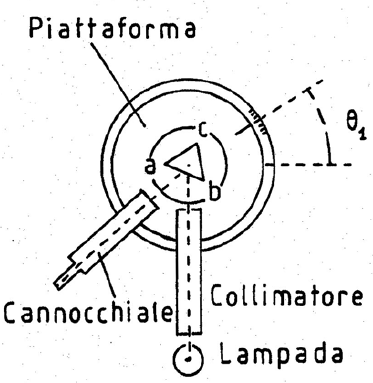
\includegraphics[width=0.5\textwidth]{apparato.png}
    \caption{Apparato sperimentale}
    \label{fig:camera_millikan}
\end{figure}

Lo spettrometro a reticolo è uno strumento utilizzato per determinare le lunghezze d’onda di una luce non monocromatica. Si articola in: 
\begin{itemize}
    \item Un collimatore che viene posto davanti alla sorgente luminosa e che rende il fascio parallelo. 
    \item  Un cannocchiale attraverso cui è possibile osservare le frange luminose. 
    \item  Un reticolo, posizionato sopra un sostegno, che separa le lunghezze d’onda del fascio incidente. 
\end{itemize}
Prima di procedere con le misurazioni è necessario regolare l’apertura del collimatore per avere un fascio di luce parallela. Per fare ciò si posiziona lo strumento in un luogo dove è possibile mettere a fuoco un oggetto posto a grande distanza. Operando sulla rotella del cannocchiale si mette a fuoco l’oggetto. Insieme all'oggetto lontano si mette a fuoco anche il crocifilo con l'apposita regolazione, utilizzato per centrare le linee dello spettro in oggetto, assicurando una maggiore precisione delle misurazioni. In questo modo si assume che i raggi incidenti siano paralleli. La posizione della rotella del cannocchiale non verrà più variata nel corso dell’esperienza.  
Si posiziona ora la sorgente di luce dietro al collimatore e il cannocchiale davanti ad esso, in modo che guardando nel cannocchiale sia possibile osservare una linea luminosa. Ruotando la rotella del collimatore si mette a fuoco la linea e si cerca di renderla abbastanza fine, per avere misure più precise, ma non eccessivamente, poiché si rischia di non riuscire ad osservare la luce diffratta ad ordini più alti.  
Dopo aver posizionato il reticolo sull’apposito supporto, è possibile procedere con l’ortogonalizzazione del reticolo, come spiegato nel paragrafo \ref{sec:ortogonalizzazione}.
\section{Precisazioni sulle misurazioni angolari}
Ogni misurazione angolare è stata presa tramite il nonio integrato nell’apparato fornito in dotazione, che consente di leggere gli angoli in gradi sessagesimali (ovvero con i sottomultipli del grado che sono rappresentati dai primi). Dunque, ogni angolo misurato tramite il nonio è stato convertito in gradi sessadecimali, esprimendo i gradi in forma decimale convertendo i primi in frazioni decimali di grado, tramite divisione per 60 dei valori misurati in primi, siccome un primo equivale ad un sessantesimo di grado. Con la stessa conversione, le incertezze sulle misurazioni degli angoli, stabilite in primi, sono state trasformate in gradi. Eventualmente, i valori angolari misurati e calcolati, così come le loro incertezze, nell’esperimento sono stati convertiti in radianti (ciò per via dell’accettazione di angoli espressi in radianti da parte dei calcolatori impiegati nel calcolo delle funzioni trigonometriche)
\[
\frac{\theta (^\circ)}{360^\circ} = \frac{\theta (\text{rad})}{2\pi}
\]
da cui:
\[
\theta (\text{rad}) = \frac{\theta (^\circ)}{360^\circ} \cdot 2\pi.
\]

\section{Procedura di ortogonalizzazione del reticolo }
\label{sec:ortogonalizzazione}
Per lo studio della dispersione cromatica tramite il passaggio attraverso il reticolo da parte di un’onda luminosa (nel caso studiato, emessa da una lampada ai vapori di mercurio) incidente perpendicolarmente rispetto al reticolo, è necessario verificare che il reticolo impiegato sia utilizzato effettivamente, con approssimazione sufficientemente buona, in condizioni di ortogonalità rispetto ai raggi luminosi che ne attraversano le fenditure. Si è stabilito di considerare accettabile un discostamento, rispetto alla condizione di ortogonalità desiderata, inferiore ai 5 primi di grado. Per ottenere l’ortogonalizzazione e misurare tale discostamento angolare, si è impiegata una lampada al sodio e si è misurata la posizione del cannocchiale dell’apparato in corrispondenza di cui la luce non ostacolata dal reticolo, che viene rimosso dalla piattaforma di lavoro, emessa della lampada al sodio risultasse centrata sul crocifilo del cannocchiale. L’incertezza sulle singole posizioni angolari misurate sono state stimate ragionevolmente pari a 2 primi, considerando le difficoltà di lettura delle tacche del nonio. Sono state eseguite 10 misurazioni della posizione angolare centrale rispetto alla lampada, di cui è stato calcolato il valor medio, per ottenerne la migliore stima, il cui errore è stato stimato come \(\frac{\sigma_theta}{\sqrt{10}}\), ottenendo: 
\[
\theta_0 = (56.123 \pm 0.011)^\circ.
\]
In seguito, dopo aver posto il reticolo sulla piattaforma e aver ruotato essa grossolanamente in modo che ad occhio il reticolo risultasse approssimativamente ortogonale al fascio luminoso, si è lavorato di precisione, misurando la posizione angolare del cannocchiale in corrispondenza della visione sul crocifilo di una delle due bande di interferenza del terzo ordine della luce emessa dalla lampada al sodio, sia sul lato destro che sul lato sinistro rispetto al centro. Siccome la condizione di perpendicolarità tra reticolo e luce incidente su di esso implica che il fenomeno debba essere simmetrico da entrambi i lati, una differenza di posizione angolare tra bande di egual ordine di una stessa lunghezza d’onda a destra e a sinistra indica un’asimmetria e quindi un discostamento dalla condizione di ortogonalità desiderata, da correggere applicando un’adeguata rotazione alla piattaforma su cui poggia il reticolo. 
Si può dimostrare, tramite considerazioni geometriche, che l’angolo \( \beta \) di cui ruotare il reticolo per raggiungere la condizione di ortogonalità, misurate le posizioni rispetto all’angolo \( \theta_0 \) della banda di diffrazione dai due lati, \( \theta_1 \) e \( \theta_2 \), è in buona approssimazione dato da:
\[
\beta = \frac{|\theta_2 - \theta_1|}{2} \cdot \left[ \frac{\cos\left(\frac{\theta_1 + \theta_2}{2}\right)}{1 - \cos\left(\frac{\theta_1 + \theta_2}{2}\right)} \right],
\]
dove \( \theta_1 \) e \( \theta_2 \) sono più precisamente le differenze tra le posizioni angolari misurate e \( \theta_0 \).
Dunque, misurati \( \theta_1 \) e \( \theta_2 \), si ruota la piattaforma di un angolo \( \beta \), nel senso che va dall’angolo misurato che è risultato minore a quello risultato maggiore. In seguito, si rimisurano \( \theta_1 \) e \( \theta_2 \), e si ricalcola \( \beta \) e si riapplica la rotazione di correzione, fino a quando \( \beta \) non risulta minore di 5 primi, in modo da considerare il reticolo nella condizione di ortogonalità richiesta per proseguire l’esperimento con approssimazione accettabile.

\section{Misurazione del passo del reticolo}
Per effettuare le misurazioni desiderate è necessario conoscere il passo del reticolo utilizzato, ovvero la distanza tra i centri di due fenditure consecutive.
Per effettuare la misura del passo del reticolo si è impiegata la stessa lampada ai vapori di sodio, le cui lunghezze d’onda delle due righe di emissione dello spettro sono note, con incertezza trascurabile, essere rispettivamente:
\[
5890 \, \text{\AA} \quad \text{e} \quad 5896 \, \text{\AA}.
\]
Il procedimento di questa misurazione è basato sull’applicazione della seguente relazione nota, che vale nel fenomeno considerato e che lega la posizione angolare \( \theta \), rispetto al centro, dei massimi di intensità luminosa di una certa lunghezza d’onda \( \lambda \) e di ordine \( k \), impiegando un reticolo di passo \( d \):
\[
d = \frac{k\lambda}{\sin(\theta)}.
\]
Da cui, l’incertezza su \( d \), a partire dall’incertezza su \( \theta \), sempre stimata pari a 2 primi, è calcolabile, grazie alla formula di propagazione delle incertezze, con il seguente calcolo:
\[
\sigma_d = \frac{k\lambda \cot(\theta)}{\sin(\theta)} \sigma_\theta.
\]
Dunque, si è misurato per 6 volte, a diversi ordini, la posizione angolare di una delle due lunghezze d’onda del sodio, in modo da calcolare 6 stime di \( d \), di cui si è calcolata la media pesata, ottenendo il risultato:
\[
d = (3.3790 \pm 0.0007) \, \mu\text{m}.
\]
È bene precisare come per ogni misurazione venga eseguita la differenza tra l’angolo misurato e la posizione angolare centrale \( \theta_0 \) di riferimento. L’incertezza sulla posizione angolare rispetto al centro così calcolata è ottenibile mediante somma in quadratura tra le incertezze dei due angoli di cui si è calcolata la differenza, per via delle regole di propagazione delle incertezze.


\section{Misurazione delle lunghezze d’onda dello spettro}

Dopo aver misurato il passo del reticolo è possibile realizzare l’obiettivo dell’esperimento, che consiste nel determinare le lunghezze d’onda che compongono lo spettro di emissione del mercurio.

Al passaggio di un’onda luminosa attraverso le fenditure del reticolo, le onde (caratterizzate da fronti sferici ma che a distanze sufficientemente grandi sono approssimabili come piani) in fase e coerenti che originano, secondo il principio di Huygens, in corrispondenza di ognuna delle fenditure interferiscono in modo completamente costruttivo nello spazio soltanto in corrispondenza di determinate posizioni angolari \( \theta_k \) (il che consente di visualizzare il centro della banda luminosa a tali posizioni angolari, dove l’intensità luminosa assume un massimo), dipendenti dal passo \( d \) del reticolo attraversato dalla luce e dalla lunghezza d’onda \( \lambda \) di questa.

Vale nello specifico la relazione già riportata sopra:

\[
d = \frac{k\lambda}{\sin(\theta)}.
\]

Pertanto, si osservano le diverse lunghezze d’onda emesse dalla lampada al mercurio venire deviate ad angoli diversi.

Misurando dunque la posizione angolare del centro di una riga di emissione di un determinato colore e ad un certo ordine \( k \), è quindi possibile calcolare la lunghezza d’onda della riga osservata tramite il calcolo:

\[
\lambda = \frac{d \sin(\theta)}{k}.
\]

L’incertezza sulla misurazione di \( \lambda \), è costituita da una componente statistica (errore su \(\theta\)) e un'altra sistematica, data dall'errore su d precedentemente calcolato:

\[
\sigma_\lambda = \sqrt{\left(\frac{\partial \lambda}{\partial d} \sigma_d\right)^2 + \left(\frac{\partial \lambda}{\partial \theta} \sigma_\theta\right)^2}.
\]

Per ogni lunghezza d’onda sono state effettuate 6 misurazioni (a diversi ordini), di cui si è eseguita una media pesata per determinarne la miglior stima e incertezza.

Di seguito riportate le lunghezze d’onda misurate per ogni colore dello spettro del mercurio che è stato possibile osservare:

\begin{table}[H]
    \centering
    \begin{tabular}{cc}
    \hline
    \textbf{Colore} & \textbf{Lunghezza d'onda} \(\lambda \, [\text{\AA}]\) \\ 
    \hline
    Rosso & \( (6240 \pm 3) \, \text{\AA} \) \\ 
    Giallo 1 & \( (5791.5 \pm 1.6) \, \text{\AA} \) \\ 
    Giallo 2 & \( (5770.8 \pm 1.7) \, \text{\AA} \) \\ 
    Verde & \( (5461.1 \pm 2.0) \, \text{\AA} \) \\ 
    Azzurro & \( (4963.5 \pm 2.7) \, \text{\AA} \) \\ 
    Indaco & \( (4359.6 \pm 1.8) \, \text{\AA} \) \\ 
    Violetto 1 & \( (4079.9 \pm 2.8) \, \text{\AA} \) \\ 
    Violetto 2 & \( (4046.3 \pm 2.2) \, \text{\AA} \) \\ 
    \hline
    \end{tabular}
    \caption{Lunghezze d'onda misurate per i diversi colori dello spettro di emissione del mercurio.}
    \end{table}
    
Le misure sono state prese a diversi ordini dal primo al quinto, e le righe di emissione sono sempre risultate sufficientemente distinguibili.

Sono state in seguito calcolate le compatibilità dei valori delle lunghezze d’onda calcolati con i valori noti forniti, ottenendo valori, in percentuale, tra il \( 19\% \) e il \( 96\% \), denotando un accordo che viene ritenuto soddisfacente.

A seguire un esempio di set di misure (per il colore “indaco”):

\begin{table}[H]
\centering
\begin{tabular}{ccccc}
\hline
\textbf{Ordine \(k\)}  & \textbf{\(\Delta \theta \)}\([\text{rad}]\) & \textbf{\(\sigma_{\Delta \theta}\)} \([\text{rad}]\) & \textbf{\(\lambda\)}  \([\text{m}]\) & \textbf{\(\sigma_\lambda\)} \([\text{m}]\) \\ 
\hline
1 & 0.1 & 0.00059 & \(4.561 \times 10^{-7}\) & \(2.0 \times 10^{-9}\) \\ 
2 & 0.3 & 0.00059 & \(4.365 \times 10^{-7}\) & \(9.6 \times 10^{-9}\) \\ 
3 & 0.4 & 0.00059 & \(4.360 \times 10^{-7}\) & \(6.1 \times 10^{-9}\) \\ 
4 & 0.5 & 0.00059 & \(4.360 \times 10^{-7}\) & \(4.3 \times 10^{-9}\) \\ 
5 & 0.6 & 0.00059 & \(4.360 \times 10^{-7}\) & \(3.1 \times 10^{-9}\) \\ 
6 & 0.7 & 0.00059 & \(4.358 \times 10^{-7}\) & \(3.1 \times 10^{-9}\) \\ 
\hline
Media & & & \(4.359 \times 10^{-7}\) & \(1.8 \times 10^{-9}\) \\ 
\hline
\end{tabular}
\caption{Set di misure per il colore indaco. La prima riga è stata rigettata poiché non coerente con le altre misurazioni.}
\end{table}


\section{Calcolo del potere dispersivo del reticolo}
Studiando il fenomeno della dispersione cromatica di un’onda luminosa che attraversa un reticolo di diffrazione, con i dati fin qui raccolti, è possibile stimare una grandezza caratteristica del reticolo, il cosiddetto potere dispersivo (che indica la capacità del reticolo di distanziare tra loro le bande di interferenza di lunghezza d’onda vicine), rapportando la distanza angolare tra i centri delle bande di interferenza delle lunghezze d’onda considerate allo scarto tra i valori delle lunghezze d’onda stesse.
Il potere dispersivo \( D \) del reticolo relativo a due lunghezze d’onda il cui scarto è pari a \( \Delta\lambda \), i cui centri delle bande di interferenza di un certo ordine risultano distanziate di una differenza angolare \( \Delta\theta \), è per definizione calcolabile come:
\[
D = \frac{\Delta\theta}{\Delta\lambda}.
\]
L’incertezza sul potere dispersivo, a partire dalle incertezze sugli scarti angolari e di lunghezza d’onda (calcolabili sommando in quadratura le incertezze su, rispettivamente, le posizioni angolari e le lunghezze d’onda di cui si calcola la differenza), si ottiene per propagazione delle incertezze dal calcolo:
\[
\sigma_D = \sqrt{\left(\frac{\sigma_{\Delta\theta}}{\Delta\lambda}\right)^2 + \left(\frac{\Delta\theta}{\Delta\lambda^2}\sigma_{\Delta\lambda}\right)^2}.
\]
Attraverso l’impiego del calcolo differenziale è possibile dimostrare come il potere dispersivo di un reticolo di passo \( d \), relativo a due lunghezze d’onda la cui media tra le posizioni angolari dei centri delle frange di interferenza all’ordine \( k \) sia \( \theta_m \), sia calcolabile come:
\[
D = \frac{k}{d \cos(\theta_m)}.
\]
Da cui l’incertezza sul potere dispersivo è ottenibile, per propagazione, dal calcolo:
\[
\sigma_D = \sqrt{\left(\frac{k}{d^2 \cos(\theta_m)}\sigma_d\right)^2 + \left(\frac{k \tan(\theta_m)}{d \cos(\theta_m)}\sigma_{\theta_m}\right)^2}.
\]
Dove l’incertezza su \( \theta_m \) è ottenibile sommando in quadratura le due posizioni angolari dei centri delle frange di ordine \( k \) delle due lunghezze d’onda considerate e dividendo per due.
Di seguito le misure del potere dispersivo del reticolo, relativo a coppie di lunghezza d’onda consecutive, ottenute tramite l’impiego della seconda formula:
\begin{table}[H]
\centering
\begin{tabular}{cc}
\hline
\textbf{Coppia di lunghezze d’onda} & \textbf{\( D \)} \([\text{rad}/\text{m}] \) \\ 
\hline
Giallo1 - Giallo2 & \( (1.0343 \pm 0.0003) \times 10^6 \) \\ 
Violetto1 - Violetto2 & \( (9.5188 \pm 0.0019) \times 10^5 \) \\ 
Rosso - Giallo1 & \( (1.04995 \pm 0.00021) \times 10^6 \) \\ 
Giallo2 - Verde & \( (1.02395 \pm 0.00020) \times 10^6 \) \\ 
Verde - Azzurro & \( (1.00128 \pm 0.00019) \times 10^6 \) \\ 
Azzurro - Indaco & \( (9.7540 \pm 0.0019) \times 10^5 \) \\ 
Indaco - Violetto1 & \( (9.5754 \pm 0.0019) \times 10^5 \) \\ 
\hline
\end{tabular}
\caption{Misurazioni del potere dispersivo del reticolo per coppie di lunghezze d’onda consecutive.}
\end{table}
A questo punto è, in linea teorica, possibile calcolare i medesimi poteri dispersivi del reticolo utilizzando la formula tramite cui si calcola il potere dispersivo attraverso il rapporto tra gli scarti delle posizioni angolari e delle lunghezze d’onda, verificandone la coerenza con i valori calcolati con la formula alternativa appena riportati.
Di seguito sono mostrati i valori ottenuti:
\begin{table}[H]
    \centering
    \begin{tabular}{ccc}
    \hline
    \textbf{D} \([\text{rad}/\text{m}] \) & \textbf{\(\sigma_D\)} \([\text{rad}/\text{m}] \) & Errore percentuale\\ 
    \hline
    \( 1.0 \times 10^6 \) & \( 1.4 \times 10^6 \) & \( 140\%\) \\ 
    \( 1.0 \times 10^6 \) & \( 4.0 \times 10^5 \) & \( 40\%\) \\ 
    \( 1.050 \times 10^6 \) & \( 2.6 \times 10^4 \)& \( 3\%\) \\ 
    \( 1.02 \times 10^6 \) & \( 4.0 \times 10^4 \) & \( 4\%\) \\ 
    \( 1.001 \times 10^6 \) & \( 2.4 \times 10^4 \) & \( 3\%\) \\ 
    \( 9.76 \times 10^5 \) & \( 1.9 \times 10^4 \) & \( 2\%\) \\ 
    \( 9.6 \times 10^5 \) & \( 4.0 \times 10^4 \) & \( 5\%\) \\ 
    \hline
    \end{tabular}
    \caption{Potere dispersivo del reticolo e relative incertezze.}
    \end{table}
    

È possibile valutare la compatibilità con le misure mostrate in precedenza, e appurare un accordo prossimo al \( 100\% \) per ogni misura. Tuttavia, si nota come le incertezze relative sulla prima e la seconda misurazione del potere dispersivo (relative rispettivamente ai due gialli e ai due violetti), condotte con il calcolo del rapporto tra \( \Delta\theta \) e \( \Delta\lambda \), risultino particolarmente elevate, ovvero rispettivamente del \(135\%\) (che priva la misura di significato) e del \(40\%\) (le incertezze relative degli altri poteri dispersivi calcolati variano invece tra il \(2\%\) e il \(4\%\)).
Le incertezze relative degli altri poteri dispersivi calcolati variano invece tra il \( 2\% \) e il \( 4\% \).
Tali risultati sono spiegabili notando come lo scarto dei due valori di lunghezza d’onda considerati sia piccolo a tal punto che l’incertezza sui due \( \Delta\lambda \) risulti dello stesso ordine di grandezza, dell’ordine di \( 10^{-9} \, \text{m} \) (nanometri), del valore del \( \Delta\lambda \) stesso, producendo quindi un’incertezza relativa elevata.
Tale problema potrebbe essere risolvibile eseguendo misure multiple (non una singola) dei \( \Delta\lambda \) all’ordine considerato e valutando l’incertezza sul \( \Delta\lambda \) con metodi statistici, a patto che si esegua un numero di misure sufficientemente elevato e sufficientemente precise.


\section{Calcolo del potere risolutivo del reticolo}
Un’altra grandezza tipica del reticolo, che è stata misurata utilizzando in questo caso la lampada ai vapori di sodio, è il potere risolutivo del reticolo, che quantifica la capacità del reticolo di risolvere lunghezze d’onda distinte, in modo che risultino separate apprezzabilmente dall’osservatore. Il criterio di Rayleigh stabilisce che due lunghezze d’onda risultano risolte dal reticolo, in modo apprezzabile per l’osservatore, nel caso in cui la posizione di massima intensità luminosa di una lunghezza d’onda oltrepassi la posizione del minimo di intensità dell’altra lunghezza d’onda.
Siano \( \lambda_1 \) e \( \lambda_2 \) due lunghezze d’onda tali che \( \Delta\lambda = \lambda_1 - \lambda_2 \) sia pari al più piccolo scarto tra due lunghezze d’onda che il reticolo è in grado di risolvere; risultino quindi le loro frange distanziate secondo la condizione limite di Rayleigh.
Il potere risolutivo del reticolo è definito come:
\[
R = \frac{\lambda}{\Delta\lambda},
\]
dove \( \lambda \) è il valor medio delle due lunghezze d’onda prese in esame.
Da questa relazione è possibile dimostrare, tramite opportune considerazioni e l’utilizzo del calcolo differenziale, che il potere risolutivo del reticolo è calcolabile come:
\[
R = Nk,
\]
dove \( N \) è il numero di fenditure illuminate del reticolo e \( k \) è l’ordine delle frange che si prendono in esame.
Dunque, due lunghezze d’onda di un certo ordine \( k \) risultano risolte, da un reticolo di \( N \) fenditure illuminate, ovvero le loro frange risultano distanziate almeno tanto quanto richiesto dalla condizione limite di Rayleigh, se si verifica:
\[
\frac{\lambda}{\Delta\lambda} \leq Nk.
\]
Dunque, si è stimato il numero di fenditure del reticolo utilizzato, in modo da calcolarne il potere dispersivo, e si è verificata la disuguaglianza sopra riportata prendendo in esame le due righe del doppietto del sodio al primo ordine (data la proporzionalità diretta rispetto all’ordine \( k \) preso in esame che è presente nell’espressione del potere risolutivo, è automatico che, nel caso in cui vengano risolte già al primo ordine, agli ordini superiori rispetto al primo le due lunghezze d’onda vengano risolte).
Il numero di fenditure del reticolo, ipotizzando che venga ognuna illuminata, è stimabile misurando la larghezza del reticolo, \( l \), e dividendo per il passo \( d \) del reticolo, che rappresenta la distanza tra due fenditure consecutive. Infine, si estrae la parte intera del rapporto:
\[
N = \text{int}\left(\frac{l}{d}\right).
\]
La larghezza \( l \) del reticolo è stata misurata con un calibro dalla sensibilità di \( 20 \, \mu\text{m} \), valore assegnato all’incertezza sistematica sulla misura della larghezza del reticolo che è stata eseguita.
L’incertezza su \( N \) si ottiene per propagazione dell’errore:
\[
\sigma_N = \sqrt{\left(\frac{\sigma_l}{d}\right)^2 + \left(\frac{l}{d^2}\sigma_d\right)^2}.
\]
Il numero di fenditure ottenuto è risultato di:
\[
N = 7318 \pm 6.
\]
Moltiplicando per l’ordine delle frange prese in esame, ovvero \( k = 1 \), il potere risolutivo del reticolo al primo ordine si stima essere:
\[
R = 7318 \pm 6.
\]
Si è inoltre calcolata la media \( \lambda \) e lo scarto \( \Delta\lambda \) delle due lunghezze d’onda del doppietto del sodio, e il loro rapporto, conoscendo i due valori delle lunghezze d’onda \( 5890 \, \text{\AA} \) e \( 5896 \, \text{\AA} \), assunte con un’incertezza di un’unità di \(\text{\AA}\).
L’incertezza su \( \Delta\lambda \) si ottiene per propagazione delle incertezze dalla somma in quadratura delle incertezze sulle lunghezze d’onda e l’incertezza su \( \lambda \) dalla stessa somma in quadratura divisa per 2.
L’incertezza sul rapporto è data da:
\[
\sigma_{\frac{\lambda}{\Delta\lambda}} = \sqrt{\left(\frac{\sigma_\lambda}{\Delta\lambda}\right)^2 + \left(\frac{\lambda}{\Delta\lambda^2}\sigma_{\Delta\lambda}\right)^2}.
\]
Si è così ottenuto:
\[
\frac{\lambda}{\Delta\lambda} = (9.8 \pm 2.3) \times 10^2.
\]
Dunque, è verificata la disuguaglianza che ci si attende di dimostrare dal momento che si osservano le due lunghezze d’onda del sodio ben risolte già al primo ordine.


\end{document}